\documentclass[output=paper]{langsci/langscibook}
\ChapterDOI{10.5281/zenodo.1407009}
\title{On lexical entries and lexical representations}
\author{Andrew Spencer\affiliation{University of Essex}}

\abstract{Lexicalist models of syntax share with lexeme-and-paradigm models of morphology the assumption that the primary unit of the lexicon is the \is{lexeme}lexeme, an abstract representation of properties unifying a set of inflected word forms. Lexicalist syntactic models (such as \isi{Head-driven Phrase Structure Grammar}, henceforth HPSG, and \isi{Sign-Based Construction Grammar}, henceforth SBCG) distinguish modelled linguistic objects from \is{description (vs. object)}descriptions of objects. A description, but not an object, can be a partial (\is{underspecification}underspecified) representation. However, a \isi{lexeme} is by definition only partially specified, being \is{underspecification}underspecified for all those morphosyntactic properties  that its word forms realize (the lexeme \lxm{dog} realizes neither singular nor plural, unlike the word forms \wf{dog, dogs}). This implies that \is{lexeme}lexemes are \is{description (vs. object)}descriptions, not objects, which is incompatible with assumptions about the \is{type hierarchy}type hierarchy for signs and the lexicon in \is{Head-driven Phrase Structure Grammar}HPSG/\is{Sign-Based Construction Grammar}SBCG. If we relax the definition of full specification to admit \is{lexeme}lexemes as objects then the question arises as to how many properties can be left unspecified. I argue for a maximally \is{underspecification}underspecified model. Even the declaration of properties for which the given class of \is{lexeme}lexemes inflects (the `\is{morpholexical signature}morpholexical signature', \textsc{morsig}) is \is{underspecification}underspecified to the extent that its contents are predictable. This entails that an inflected word form of a \isi{lexeme} can be defined only after the \textsc{morsig} attribute is specified. Derivation, a \is{lexeme}lexeme-to-lexeme mapping,  can therefore be defined over the same maximally \is{underspecification}underspecified \is{lexical representation}lexical representations, whose inflection is then typically governed by a different \is{morpholexical signature}morpholexical signature (e.g. when the derivation changes word class). All such specifications are given by \is{default}default statements, which are overridden for irregular items. Verb-to-adjective \is{transposition}transpositions \is{participle}(participles) are members of the verb's paradigm yet inflect according to the adjectival paradigm (the `adjectival \is{\textsc{representation} (feature)}representation' of a verb). This gives the effect of a `\is{lexeme}lexeme-within-a-lexeme', posing a challenge for \is{lexeme}lexeme-and-paradigm models. I present an analysis in which the definition of the \isi{participle} is driven by a feature \is{\textsc{representation} (feature)}\textsc{representation}. This (re-)defines the \textsc{morsig} attribute, creating a representation which is identical to that of an adjective, while remaining part of the verb's paradigm. I discuss some of the implications of this analysis for  lexical relatedness, the lexical \is{type hierarchy}type hierarchy of \is{Sign-Based Construction Grammar}SBCG and the morphology-syntax interface.}

\maketitle
\begin{document}
\selectlanguage{english}



%\input{lspboiler}

\section{Introduction} \label{sec:Spencer:introduction}


The notion of word is by definition central to lexicalist models of syntax, so one would imagine that morphology, too, would occupy a central place in the construction of such models. However, there is as yet surprisingly little consensus between morphologists and syntacticians over fundamental aspects of word structure and the relations between words and syntax or semantics. In addition, I will argue that there is a systematic unclarity in conceptualizations of wordhood even amongst those of us who accept the primacy of the \isi{lexeme} notion and its role in morphosyntax (`\is{lexeme}lexeme-and-paradigm' models). One central ontological question is `what kind of a thing is a word?' The problem is that, whereas inflected word forms can be regarded as `concrete' linguistic objects which combine with each other to form phrases (another type of object), \is{lexeme}lexemes are by their nature more abstract: they are ultimately representations which unite a set of related inflected word forms without themselves being a form. They are therefore \is{underspecification}underspecified representations, in the sense that they are not specified for the various morphosyntactic properties their word forms realize. The dictionary is a set of \is{lexeme}lexemes, so it, too, is an abstract construct.

The question of what \is{lexeme}lexemes are is made more acute when we examine a somewhat neglected, but theoretically and conceptually important, type of lexical relatedness, the (true) \is{transposition}transposition, illustrated in this paper by the \ili{Russian} deverbal \is{participle}participle. A \isi{participle} is the adjectival `\is{\textsc{representation} (feature)}representation' \citep{Haspelmath1996} of a verb. As such, it is part of the paradigm of a verb and yet it inflects exactly like an adjective and demonstrates much of the external syntax of an adjective (a true \isi{participle} is used principally as an attributive modifier to a noun). Shifting morphosyntactic category in this fashion is characteristic of derivation, i.e. \isi{lexeme} formation, yet a true \isi{participle} (that is, a \isi{participle} that has not undergone lexicalization, or some other process of grammaticalization) is not an autonomous \is{lexeme}lexeme, independent of its verb base, any more than the past tense or the infinitive form of a verb is an autonomous \is{lexeme}lexeme. The \isi{participle} thus gives the appearance of being a `\is{lexeme}lexeme-within-a-lexeme', posing obvious difficulties for any simple characterization of \is{lexeme}lexeme-and-paradigm inflectional morphology, and especially to the \is{inferential-realizational}inferential-realizational (I-R) class of models in %
%Stump's (2001) 
\citepos{Stump01:book} %
%Stump
%
typology.

\begin{sloppypar}%
In this paper I investigate some of these questions against the backdrop of the class of \is{inferential-realizational}I-R models called Paradigm Function Morphology (PFM: \citealt{Stump01:book,Bonami:Stump16:PFM}). Specifically, I will assume the overall architecture of a model of lexical relatedness proposed in \citet{Spencer13}, \isi{Generalized Paradigm Function Morphology} (GPFM). I confront the proposals  about \is{lexical representation}lexical representations and lexical relatedness made in \is{Generalized Paradigm Function Morphology}GPFM with influential proposals put forward within the variant of \is{Head-driven Phrase Structure Grammar}{HPSG} developed by \citet{Sag12}, Sign-Based Construction Grammar (\is{Sign-Based Construction Grammar}SBCG). I argue that the \is{Head-driven Phrase Structure Grammar}HPSG/\is{Sign-Based Construction Grammar}SBCG conception of the \isi{lexeme} conceals important conceptual inconsistencies. In particular, a \isi{lexeme} can only be described by a feature structure (FS) that is partially specified. However, this means that technically a \isi{lexeme} is just a \is{description (vs. object)}description and not an object. Yet the architecture of the \is{Head-driven Phrase Structure Grammar}{HPSG} lexicon demands that \is{lexeme}lexemes be bona fide linguistic objects, not \is{description (vs. object)}descriptions of objects.\end{sloppypar}


If we simply declare the \is{lexeme}lexemes as objects then the question arises as to how much the \isi{lexeme} can be \is{underspecification}underspecified. Building on the \is{default}defaults-based \is{Generalized Paradigm Function Morphology}GPFM model I argue that a \isi{lexeme} is best regarded as a \emph{maximally} \is{underspecification}underspecified object, bearing all and only those properties which are not predictable from \is{default}default specifications.%
\footnote{This corresponds to \citeauthor{Sag12}'s \citeyear{Sag12} notion of \is{listeme}listeme.
The \isi{listeme}  has a somewhat unclear status in \is{Sign-Based Construction Grammar}SBCG, but Sag explicitly describes it as a \is{description (vs. object)}description and not an object, so it is not a perfect correspondent to the conception of \isi{lexeme} proposed here.
} %
I show how the maximally \is{underspecification}underspecified \is{lexemic representation}lexemic representation can help solve the question of the status of \is{transposition}transpositions such as \is{participle}participles.

I make a number of background assumptions.

\begin{itemize}

\item	A dictionary is a list of \is{lexeme}lexemes.

\sloppy
\item	Inflectional morphology operates according to \is{inferential-realizational}I-R principles and defines a para\-digm for each class of \is{lexeme}lexemes, each cell of which is occupied by a pair $\langle$ω,σ$\rangle$ for the set σ of morphosyntactic properties realized by the word form ω.
\fussy 

\item	A fully specified representation of a \isi{lexeme} includes a specification of a set of syntactic properties, a semantic representation (which for convenience I take to be a simplified form of Lexical Conceptual Structure, \citealt{Jackendoff90}) and a unique identifier, variously called the Lexical Identifier (\textsc{lid}), the Lexical Index, or  the Lexemic Index (\textsc{li}). (This is comparable in function to the lexicographer's lemma.)

\item
The syntactic properties of a \isi{lexeme} include a specification of its \isi{argument structure} (\textsc{arg-st}).

\item
The \textsc{arg-st} attribute of a \isi{lexeme} includes a \isi{semantic function role} %
%(SF role, Spencer 2013)
\citep[SF role,][]{Spencer13}%
%Spencer
%
, canonically R for nouns, E for verbs and A for adjectives
\end{itemize}

The chapter is structured as follows. %
I open by outlining four possible ways of representing \is{lexeme}lexemes, the fourth of which relies heavily on the device of \is{default}defaults and overrides operating over a maximally \is{underspecification}underspecified entry. The next section addresses  the question of whether a \isi{lexeme} can be regarded as an object or not, %
and how many of its properties can be \is{underspecification}underspecified.

In \S\ref{sec:Spencer:morsig}  I turn briefly to the model of lexical representation proposed in %
%Spencer (2013)
\citet{Spencer13}%
%Spencer
%
, and specifically to the way in which an inflectional feature declaration (\textsc{morsig}, `\is{morpholexical signature}morpholexical signature') can be defined and deployed in a \is{default}defaults-based model of lexical representation.
Against this background \S\ref{sec:Spencer:lexrelli} addresses the architecturally important question of the place of \is{transposition}transpositions such as deverbal \is{participle}participles. These are an important test case because they raise questions of \is{lexeme}lexemic identity and category membership: the \isi{participle} behaves as a \is{quasi-lexeme}`quasi-lexeme', without being the output of derivational \isi{lexeme} formation proper. I deploy an attribute \is{\textsc{representation} (feature)}\textsc{representation} to define \is{transposition}transpositions. I discuss the way that the adjectival inflectional paradigm can be incorporated into the paradigm of a verb by appropriate use of the \textsc{morsig} attribute. I illustrate with a description of the \ili{Russian} \is{participle}participial system. I contrast the behaviour of true \is{participle}participles with that of \is{transpositional lexeme}transpositional lexemes %
%(Spencer 2013, 2016)
\citep{Spencer13,Spencer16:MorphMetatheory}%
%Spencer;Spencer
%
, which are derived autonomous lexemes formed from \is{transposition}transpositions such as \is{participle}participles.

In \S\ref{sec:Spencer:lextypes} I ask how \is{transposition}transpositions might be incorporated into a multiple inheritance hierarchy but note two problems. First, multiple inheritance hierarchies are not straightforwardly capable of distinguishing, say, the adjectival \is{\textsc{representation} (feature)}representation of a verb \is{participle}(participle) from the verbal \is{\textsc{representation} (feature)}representation of an adjective (inflecting predicative adjective). Second, there is in any case virtually no discussion in the morphological literature of \is{transposition}transpositions and hence no consensus on how their morphological properties should be accounted for.
I conclude with a tentative list of questions which arise from the discussion.


I will close this introduction with a terminological note. I shall simplify discussion wherever possible by assuming the correctness of my approach and taking the \isi{lexeme} to be effectively identical to its \is{description (vs. object)}description. That is, a \isi{lexeme} is a dictionary entry, an abstract \is{underspecification}underspecified representation, which we can think of as a meta-representation, unifying the concrete representations in the complete set of its word forms. The obvious synonym for `dictionary entry' is  `\is{lexical entry}lexical entry'. However, in constraints-based syntactic models the notion of `\is{lexeme}lexeme' is rather poorly developed, and the term `\is{lexical entry}lexical entry' is often (though not invariably!) used to refer not to the abstract object listed in a dictionary but rather to a concretely instantiated inflected word form of a \is{lexeme}lexeme. This terminological ploy is confusing, but is now ingrained.
Following \citet{Dalrymple:etal15:morphology}, I shall therefore  adopt the term `lexemic entry' for the standard lexicographic notion of dictionary entry. I will avoid the term `\is{lexical entry}lexical entry' and refer to the representation (fully or partially specified) of an inflected form as the \is{lexical representation}lexical representation of that word form. This is more than a question of mere terminology, especially in \is{Head-driven Phrase Structure Grammar}HPSG, but proper evaluation of the issues would require a separate study.

 %%%%%
 %%%%%%

%The nature of the lexeme
\section{The nature of the \isi{lexeme}}	\label{sec:Spencer:nature}

In principle there are a good many ways  in which dictionary entries can be represented. It will be useful to consider four of these. The first possibility is to list every inflected form separately with a complete specification of all its properties, whether idiosyncratic or predictable. This will include (i) all the morphological properties, such as inflection class, (ii) syntactic properties such as \isi{argument structure}, including the \is{semantic function role}SF (semantic function) roles, valence, selection, collocation, lexicosyntactic class features and others, together with (iii) contextual properties or properties relating to usage such as register, connotations, and other, not strictly linguistic, properties that a competent user would be expected to know about the word (what is sometimes called `encyclopaedic information', though this term is difficult to pin down).  I shall call this mode of representation the \emphterm{unindexed full word form listing} model. Some psycholinguistic models of the mental lexicon appear to have essentially this structure. It does not define a dictionary entry in any direct sense because every word form of every \isi{lexeme} has the same representational status as any other:
\textex{dog} and \textex{dogs} are only marginally more related to each other on this model than are \textex{dog} and \textex{dig} or \textex{dogs}  and \textex{geese}.

The unindexed full word form listing  model  effectively excludes any standard understanding of the notion of dictionary entry, therefore. However, it would be possible to reconstruct the traditional notion of dictionary entry by providing all the forms that unite under a given \isi{lexeme} with a unique \emphterm{lexemic index}. Thus, \textex{dog, dogs} would both have the index \lxm{dog}, distinct from that of \textex{dig} (\lxm{dig}) or \textex{geese} (\lxm{goose}). This would then define our second model of lexical representation, which I will call the \emphterm{indexed full word form listing} model. The \textsc{li} would have to be a secondary property associated with each component of a lexemic entry, \textsc{form}, \textsc{syn}, \textsc{sem}. At the level of \textsc{form} this would mean indexing the \is{lexeme}lexeme's root, its various stem forms and all its inflected forms (unless these were able to inherit the \textsc{li} of their stems). At the level of \textsc{syn}, \textsc{sem} each individual subattribute (syntactic class, \isi{argument structure} or whatever, depending on one's syntactic assumptions) would be furnished with the same \textsc{li}, as would the basic meaning or lexical conceptual structure and any other aspects of meaning. This use of a lexemic index is very  similar to that proposed by \citet{jackendoff97} and integrated into the Simpler Syntax model \citep{Culicover:Jackendoff05}, though their model makes rather different assumptions about the structure of inflected words because it retains the morphemic concept and therefore is not strictly speaking \isi{lexeme}-based.

%%%%%%

These first two models share the property that all inflected word forms are fully listed. In such models there is effectively no morphology defining the lexical relatedness that holds between word forms of the same \is{lexeme}lexeme. In order to capture formal similarity/iden\-tity between word forms it would therefore be necessary to postulate lexical redundancy rules (\citealt{Jackendoff75,Bochner93}) or inflectional templates
\citep{AckermanBlevinsMalouf09}.

The third model I shall call the \emphterm{fully specified lexemic entry} model. The term `fully specified' refers to the fact that on this   model (along with  the previous two models)  the lexemic entry includes fully predictable information about the \textsc{form}, \textsc{syn}, \textsc{sem} representations as well as unpredictable, idiosyncratic information. For instance, if all syntactic nouns in the language are also morphological nouns (i.e. if the language lacks category mixing with respect to the noun class) then the property of inflecting as a noun, that is, being a morphological noun, can be deduced from the \textsc{syncat} label. However, under the fully specified lexemic entry model such a word would still be given the attribute [\textsc{morcat}~\textit{noun}] or the equivalent as part of its \textsc{form} representation. Where this third model differs from the previous two is in the important assumption that (regularly) inflected word forms are not included as part of the lexicon as such. Rather, such a model follows lexicographic tradition in abstracting away from inflected word forms, instead, defining  them by means of a separate `inflectional engine', such as PFM. On the fully specified lexemic entry model, the \is{lexeme}lexeme-as-dictionary-entry is accorded a special ontological status, that of a linguistic object. Depending on how such a model is implemented formally it may or may not be necessary to individuate dictionary entries by means of the arbitrary \textsc{li} attribute. However, traditional lexicography certainly makes use of something very close to an \textsc{li} in the form of a lemma or headword. An arbitrary label of this sort  appears to be the most natural way of individuating entries.

The fourth model of lexical representation is the \emphterm{\is{underspecification}underspecified lexemic entry } model, argued for in %
%Spencer (2013)
\citet{Spencer13}%
%Spencer
%
. This model deploys the logic of \is{default}default inheritance to abstract away fully predictable lexical information. The \is{lexemic representation}lexemic representation in this case includes just the information that cannot be inferred by \is{default}default from other aspects of the representation or from other facts in the grammar of the language. Thus, in our previous example, if the specification [\textsc{morcat}~\textit{noun}] is fully predictable from the specification [\textsc{syncat}~\textit{noun}] then the \textsc{morcat} specification need not be stated in the lexemic entry itself (indeed, there need be no mention of the attribute \textsc{morcat} at all).

To see how the \is{underspecification}underspecified \isi{lexical entry} model might define dictionary entries, consider a word such as \lxm{tree}. This minimally has to specify a phonological form for the basic stem form (root), \textsc{stem$_0$} = /triː/, as well as  minimal information about the kind of meaning the word has. As far as morphosyntax and especially inflection  is concerned it hardly matters, of course, what kind of a thing a tree is (much less where to draw the line between trees and bushes). Also, the difference between abstract and concrete denotations seems to have little grammatical import, in \ili{English}. However,  it is important to know that \lxm{tree} denotes some type of \textit{Thing} and that it is countable, in contrast to words such as \lxm{vegetation}, or \lxm{wood} (in the sense of `material coming from a tree'). Informally, we can distinguish count \textit{Things} and mass \textit{Things} with a subscript: \textit{Thing\textsubscript{c}}/\textit{Thing\textsubscript{m}}. However, for \ili{English} we should also have some way of representing the fact that \lxm{tree} (and \lxm{idea}) denotes something which is not a sexed higher animal, such as a person or a horse and which therefore can only be referred to as \wf{it}, not as \wf{s/he}. In languages which distinguish a `vegetable' gender (e.g.\il{Bininj-Gunwok} Bininj-Gunwok) we might need to indicate the fact that \lxm{tree} (and perhaps \lxm{vegetation} but not \lxm{idea}) denotes a kind of plant. In other languages with semantically-driven gender other distinctions would have to be made. These observations hold for the determination of inflectional properties. However, for a specification of derivational morphology it is often necessary to appeal to very subtle nuances of meaning \citep{Fradin03b}.

The point of this discussion of lexical semantics is that once the right semantic properties are fixed much of the rest of the \is{lexemic representation}lexemic representation can be deduced by \is{default}default. Thus, if an \ili{English} \isi{lexeme} belongs to the \textit{Thing} ontological category (as opposed to the category \textit{Event} or \textit{Property}) then by \is{default}default it will be a noun, with an \isi{argument structure} that includes the \is{semantic function role}SF role R.  A syntactic noun  will also be a noun morphologically, and if it is of subcategory \textit{Thing\textsubscript{c}} it will have  a singular and plural form. This is more than just a modern version of the notional parts-of-speech theory, however.  Being \is{default}defaults, all these inferences can, of course, be overridden by more specific lexical stipulations.  Thus, a noun such as \lxm{journey} is ontologically an \textit{Event} but grammatically it is a noun, so that the inference from \textit{Event} to \is{semantic function role}SF role E to [\textsc{syncat}/\textsc{morcat}~\textit{verb}] is overridden in the lexemic entry (for instance, by stipulating that its \is{semantic function role}SF role is a simplex R). %
 Moreover, in many languages there will be non-\is{default}default morphological information to stipulate in addition to the phonology of the root. For instance,  the \ili{Russian} noun \lxm{stolovaja} `canteen; dining room' is a noun syntactically, but it has the morphology of a (feminine gender) adjective, thus its [\textsc{morcat}~\textit{adjective}] value cannot be inferred from its [\textsc{syncat}~\textit{noun}] value and has to be stipulated in the lexemic entry in some way.
 In some cases, not all  \isi{argument structure} or complementation properties can be deduced from the semantic representation so those would need to be specified lexically. Some of the contextual properties of a \isi{lexeme} such as special register, connotations, or other details of usage may also diverge from the \is{default}default and will therefore have to be recorded in the \is{lexeme}lexeme's entry.
But the limiting case of a lexical representation in the \is{underspecification}underspecified lexemic entry model is a pure pairing of basic meaning with the form of the root %
(what %
%Sag 2012 
\citealt{Sag12} %
%
refers to as a \is{listeme}`listeme'; see \S\ref{sec:Spencer:objordesc})
%\citep[what ][ refers to as a \is{listeme}`listeme'; see \S\ref{sec:Spencer:objordesc}]{Sag12}%
%Sag
%
.



%%%%%%%%%%%%%%%%%%
%%%%%%%%%%%%%%%%%%%

%%%%%%%%%%%%%%%%%%
%%%%%%%%%%%%%%%%%%%

%Lexemes as objects or descriptions

\section{Lexemes as objects or \is{description (vs. object)}descriptions} \label{sec:Spencer:objordesc}


The principal question to be addressed in this paper is: what kind of a representation is a dictionary (lexemic) entry? Specifically, is it a linguistic object in its own right? In this section I discuss the answers proposed in %
%Sag's (2012) 
\citepos{Sag12} %
%Sag
%
%\nocite{Sag12} 
 summary of \is{Sign-Based Construction Grammar}SBCG.

In \is{Sign-Based Construction Grammar}SBCG, as in \is{Head-driven Phrase Structure Grammar}{HPSG} generally, a distinction is drawn between linguistic objects and the representational technology used to describe those objects, notably feature structures (FSs) or attribute-value matrices (AVMs). An inflected word form, for example, is a linguistic object, but it can be described in various ways, including partial feature descriptions which \is{underspecification}underspecify certain aspects of the representation. A linguistic object proper, however, cannot be thus \is{underspecification}underspecified. This means, for instance, that Sag's  \is{listeme}listeme, the barest possible representation of a lexemic entry, must be a \is{description (vs. object)}description, not an object in its own right.

Sag \page{98} introduces the notion of the \isi{lexeme} into the model, giving it a special place in the \is{type hierarchy}type hierarchy of signs shown in Figure \ref{fig:Spencer:types}. This hierarchy defines the \isi{lexeme} as a lexical sign, just like a word form. However, word forms appear as parts of syntactic phrases which can ultimately be pronounced, and so they count as linguistic expressions. A \isi{lexeme} cannot be pronounced. This is not because it is some kind of `covert expression', however (like \textit{gap} and \textit{pro} in Sag's \is{type hierarchy}type hierarchy). A \isi{lexeme} is an altogether different kind of sign, in fact, a unique \is{type hierarchy}type given the hierarchy in Figure \ref{fig:Spencer:types}.

\begin{figure}
\begin{centering}
\itshape

	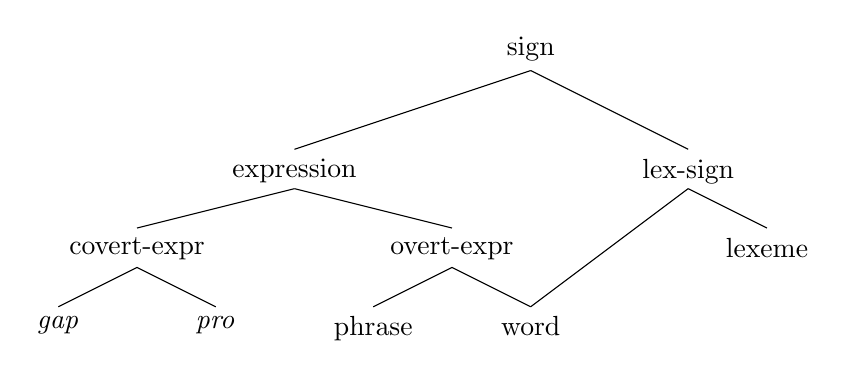
\begin{tikzpicture}

%\node[anchor=center] at (0,0) {};
\draw (0,0) node[above]{sign};

\draw (0,0) -- (2,-1);
\draw (2,-1) node[below]{lex-sign};

\draw (0,0) -- (-3,-1);
\draw (-3,-1) node[below]{expression};

\draw (2,-1.5) -- (3,-2);
\draw (3,-2) node[below]{lexeme};

\draw (2,-1.5) -- (0,-3);
\draw (0,-3) node[below]{word};

\draw(-3,-1.5) -- (-1,-2);
\draw  (-1,-2) node[below]{overt-expr};

\draw(-3,-1.5) -- (-5,-2);
\draw (-5,-2) node[below]{covert-expr};

\draw(-1,-2.5) -- (0,-3);
\draw(-1,-2.5) -- (-2,-3);
\draw  (-2,-3) node[below] {phrase};

\draw(-5,-2.5) -- (-4,-3);
\draw (-4,-3) node[below] {\textit{pro}};

\draw(-5,-2.5) -- (-6,-3);
\draw  (-6,-3) node[below]{\textit{gap}};

	\end{tikzpicture}

 \caption{ %
%Sag's (2012) 
\citepos{Sag12} %
%Sag
%
\is{type hierarchy}type hierarchy} 			\label{fig:Spencer:types}
\end{centering}
\end{figure}




\begin{figure}
\begin{center}
%\begin{tikzpicture}
%\node(0.5,0) {



\framebox{
\begin{avm}
  \[\asort{sintrans-v-lxm}
  phon	&/læf/\\
  form	&\<\upshape\itshape laugh\>\\
  arg-st	&\<NP$_{i}$\>\\
  syn	&\[\asort{syn-obj}
  		cat	&\[\asort{verb}
  				select &none\\
  				vf	&psp\\
  				xarg	&NP$_{i}$\\
  				lid	&\<\[\asort{laughing-fr}
  						label	&l$_{1}$\\
  						sit	&s\\
  						s-srce	&i\]\>\\
  		mrkg	&unmk\\
  		val	&\<NP$_{i}$\>\\
  			\]
  	  \]\\
  sem	&\[\asort{sem-obj}
  	ind	&s\\
  	ltop		&l$_{1}$\\
  	frames	&\<\[\asort{laughing-fr}
  				label	&l$_{1}$\\
  				sit	&s\\
  				s-srce	&i\]\>	\]
  \]
\end{avm}
}
%};
%\draw (-5.5,-7.5) rectangle (6,7);
%\end{tikzpicture}
\caption{ %
%Sag's (2012: 111) 
\citeposp{Sag12}{111} %
%Sag
%
representation of the \isi{lexeme} \lxm{laugh}} \label{fig:Spencer:laugh}
\end{center}
\end{figure}

Sag provides examples of representations of word forms from \ili{English} (plurals, past tense forms) and in his Fig. 6 (p. 101), here reproduced as Figure \ref{fig:Spencer:laugh}, he gives the example of the \isi{lexeme} \lxm{laugh}.  Notice that this representation actually seems to specify the word form \wf{laughed}, in that it bears the feature  [\textsc{vform}~\textit{psp}]. It is worth citing Sag's  justification for this choice of representation:


\begin{quotation}
 [T]he value \textit{psp} illustrated here [\ldots] represents an arbitrary expositional choice \textemdash{\ } any value of \textsc{vform} would satisfy the requirements imposed by the \textit{laugh} \is{listeme}listeme. And each such choice gives rise to a family of well-formed FSs licensed by that \is{listeme}listeme.
 \citep[99]{Sag12}
\end{quotation}

\noindent
Sag here appeals to the \lxm{laugh} \is{listeme}listeme. In \is{Sign-Based Construction Grammar}SBCG a \isi{listeme} \emph{licenses} modelled linguistic objects. This  means  that it places restrictions on what properties a modelled object or sign may have \page{105}. Another way of characterizing the \isi{listeme} is as \textquotedblleft a \isi{lexeme} \is{description (vs. object)}description in the lexicon\textquotedblright{} \page{107}.

The type \textit{\is{lexeme}lexeme} plays a central role in \is{Sign-Based Construction Grammar}SBCG, in that it is the starting point for all morphology (Sag is here following PFM and related models). Inflection and derivation are modelled by means of morphological functions. An inflectional rule such as the \ili{English} preterite (past tense) is modelled by a \textit{preterite-cxt}, whose mother is the past tense form and whose daughter is the \isi{lexeme} whose past tense form is being defined. A derivational rule is given by a construction whose mother is the derived \isi{lexeme} and whose daughter is the base \is{lexeme}lexeme.

Sag summarizes the morphological functions by saying \page{113} that they express \textquotedblleft <\ldots{}> the relation between the forms of two \is{lexeme}lexemes or the relation between the form of a \isi{lexeme} and the form of a word that realizes that \is{lexeme}lexeme.\textquotedblright\ This sounds like an expression of conventional wisdom in \is{lexeme}lexeme-based morphology, but it hides a serious conceptual flaw. This  centres around the way that Sag's formulation uses the term `form'. The problem is apparent from Sag's description of the \isi{lexeme} \lxm{laugh}. He is obliged to provide this representation with an arbitrary inflectional feature specification, in effect defining not the \isi{lexeme} as such but one of its inflected forms. This is because a \isi{lexeme} is meant to be a modelled object, a subtype of \textit{sign}, and a linguistic object must be fully specified. But the whole point of defining a \is{lexeme}lexemic level of representation is to abstract away from actual (concrete) word forms. This means that the \isi{lexeme} is effectively a \is{description (vs. object)}description, in fact a partial \is{description (vs. object)}description, of the full set of word forms. But that is completely incompatible with Sag's \is{type hierarchy}type hierarchy and, indeed, with any coherent interpretation of the \is{Head-driven Phrase Structure Grammar}{HPSG} lexicon.



Given this reasoning we seem to have two logical courses of action. Either we can re-construct the \is{Head-driven Phrase Structure Grammar}{HPSG} lexicon without recourse to the type \textit{\is{lexeme}lexeme}, or we can redefine the notion of linguistic object in such a way as to make a dictionary entry a kind of modelled object, even though it appears to be \is{underspecification}underspecified. I shall adopt the second approach.

I propose to treat the lexicon as more than just a convenient descriptive fiction, as would be implied by  a strict application of the object$\sim$\is{description (vs. object)}description distinction. Rather, I take the lexicon to be a network of mentally represented (or representable) objects which can be defined and described by FSs just like (utterable and unutterable) linguistic expressions.

By simply declaring a dictionary (lexemic) entry to be a kind of object we solve the immediate problem: the \isi{lexeme} can remain a type of sign, and can be a supertype of other signs. Its unusual position in being partially \is{underspecification}underspecified is now reflected in the \is{type hierarchy}type hierarchy: only the \textit{expression} \is{type hierarchy}type has to be fully specified, a lexical sign may be only partially specified (\textit{\is{lexeme}lexeme}), though when a lexical sign is also a sub\is{type hierarchy}type of \textit{expression} (\textit{word}) it, too, can, and must, be fully specified.

Now, once we admit the possibility of an \is{underspecification}underspecified entity as an object in the linguistic ontology we are immediately faced with two sets of questions. The most general of these is `are there other linguistic objects which can be less than fully specified? Can \emph{any} partially specified representation be interpreted as a modelled object? If so, then what is the content of the original object$\sim$\is{description (vs. object)}description distinction?'' %
It seems that we should not be allowed to postulate such objects except in very special circumstances. But if we admit \is{lexeme}lexemes as less than fully specified objects  what prevents us from postulating entirely arbitrary \is{type hierarchy}types? The simplest answer is to say that it is an architectural (i.e. stipulated) property of linguistic
expressions that they be fully specified. However, whether this is really true may depend on how we perceive linguistic specification. Presumably, an object of type \textit{word} such as \textex{dogs} is to be regarded as a fully specified object and not a \is{description (vs. object)}description, even when, for instance, its intonation and other prosodic characteristics are not specified. But in the strictest sense a word form remains partially \is{underspecification}underspecified until its full phonetic realization is given. Indeed, the same is true of sentences, which can be uttered with a very wide variety of affective intonation contours even when realizing one and the same set of discourse or information-structure functions.

The second question is more immediately relevant: if we are to admit as an object a \isi{lexeme} \is{underspecification}underspecified for its inflection properties, how much further can we go with the \is{underspecification}underspecification? For instance, we might want to say that our \isi{lexeme} \lxm{laugh} is \is{underspecification}underspecified for its inflectional properties by virtue of bearing the attribute values [\textsc{tense}  u, \textsc{vform}  u, \textsc{subjagr}  u, \ldots{}] or whatever, where `u' means `not yet specified value', or we may wish to make the more radical proposal that \lxm{laugh} lacks the actual attributes [\textsc{tense}, \textsc{vform}, \textsc{subjagr}, \ldots{}]. This may turn out to be little more than a matter of notational convention, but in a more radical vein we can ask why we can't regard Sag's maximally \is{underspecification}underspecified \isi{listeme} as a \is{default}default \isi{lexeme} object. %
In other words, can we not adopt the \is{underspecification}underspecified lexemic entry model for dictionary entries, as proposed in %
%Spencer (2013)
\citet{Spencer13}%
%Spencer
%
?  We will see that the question  assumes particular importance in \is{default}defaults-based models of morphology such as PFM, where the \isi{lexeme} concept finds its most elaborated implementation, and especially \is{Generalized Paradigm Function Morphology}GPFM, where \is{default}defaults define all aspects of lexical representation. %
 Before turning to  a consideration of the \isi{lexeme} concept in such  models I first discuss an important but generally neglected aspect of lexical representation and its relation to inflectional morphosyntax.

%%%%%%%%%%

%%%%%%%%%%%%%%%%%%%%%%%%%%%%%%%

%The morpholexical signature (\textsc{morsig})

\section{The \is{morpholexical signature}morpholexical signature (\textsc{morsig})} \label{sec:Spencer:morsig}


A \isi{lexeme} of a given morpholexical class, such as `noun', will (typically!) inflect for properties particular to that class (say, \textsc{number, case, definiteness, possessor agreement}) and may have intrinsic properties which determine its morphosyntax, such as \textsc{gender}. The actual set of properties is stipulated for each language, so a grammar has to include a declaration of that set. In the \isi{Generalized Paradigm Function Morphology}(GPFM) model of %
%Spencer (2013) 
\citet{Spencer13} %
%Spencer
%
I refer to this declaration as the \emphterm{\is{morpholexical signature}morpholexical signature} (\textsc{morsig}). In \is{Generalized Paradigm Function Morphology}GPFM the \textsc{morsig} attribute is itself treated as a \is{default}default property with respect to lexemic entries\slash{}representations. By this I mean that the properties which make up the \textsc{morsig} are true of every regular \isi{lexeme} of the given class, so it would be redundant to specify that information in the lexemic entry itself.

In %
%Spencer (2013) 
\citet{Spencer13} %
%Spencer
%
I treat the \textsc{morsig} as a value of the \textsc{form} attribute, i.e. as a morphological property of a \is{lexeme}lexeme, but this is an oversimplification. It is well-known that the set of features needed to define a \is{lexeme}lexeme's syntactic distribution, and the set of grammatical meanings expressed by inflected word forms, are often at variance with the set of features needed to define the inflected morphological forms themselves.   The most obvious mismatches are found in \is{periphrasis}periphrases. We often find that   the morphological form of one of the elements of the construction bears properties which contradict the feature content expressed by the \is{periphrasis}periphrasis as a whole.
Elsewhere, the morphological element may be morphomic and therefore not associated with any meaning, or the \is{periphrasis}periphrasis may express a meaning in the manner of an idiom, so that no part of it can sensibly be associated with the meaning of the \is{periphrasis}periphrasis as a whole \citep{Brown12c}. \is{periphrasis}Periphrasis therefore motivates a distinction between \is{m-feature}\mbox{m-features} and \is{s-feature}\mbox{s-features} (mnemonically, morphological/syntactic features, \citealt{Sadler:Spencer01}). Similarly,  Stump has argued for a modification of the original Paradigm Function Morphology (PFM) model, `PFM1' \citep{Stump01:book}, in favour of a model, `PFM2', which draws a distinction between\is{paradigm!form paradigm} \textsc{form} and \is{paradigm!content paradigm}\textsc{content} paradigms, on the basis of mismatches such as syncretisms, deponency and a variety of others %
%\nocite{Stump02:paradigmlinkage,Stump06:heteroclisis,Stump16,Stump16:MorphMetatheory}%
%(Stump 2002, 2006, 2016a,b)
\citep{Stump02:paradigmlinkage,Stump06:heteroclisis,Stump16,Stump16:MorphMetatheory}%
%Stump;Stump;Stump
%
. The obvious way to capture such distinctions in \is{lexical representation}lexical representations is to assume that there is a \textsc{syn}|\textsc{morsig} attribute which is mapped to a \textsc{form}|\textsc{morsig} attribute by means of a function,  Stump's `paradigm linkage'. By default, paradigm linkage is the identity function, in the sense that the \is{paradigm!form paradigm}{\textsc{form} paradigm} or \isi{m-feature} set is identical to the \is{paradigm!content paradigm}\textsc{content} paradigm/s-feature\is{s-feature} set.

In \is{Generalized Paradigm Function Morphology}GPFM the relation between the most highly \is{underspecification}underspecified \is{lexical representation}lexical representation and a fully specified word form is mediated by two sets of functions. The second of these is effectively identical to the \isi{paradigm function} of PFM2. It maps a pairing of $\langle$$\mathcal{L}$,σ$\rangle$, for \textsc{li} $\mathcal{L}$, feature set σ, to a pair  $\langle$ω,σ$\rangle$, where ω is the corresponding inflected word form. This function is, however, only defined for a complete and coherent feature set. In other words the function cannot be defined for a representation which lacks a specification of those features for which the \isi{lexeme} inflects, that is, the \textsc{morsig}. Therefore, to be inflectable the \is{lexeme}lexeme's \textsc{morsig} attribute needs first to be specified \is{Inflectional Specifiability Principle}%
%(\emph{Inflectional Specifiability Principle}, Spencer 2013: 199)
\citep[\emph{Inflectional Specifiability Principle},][199]{Spencer13}%
%Spencer
%
. This is achieved by the first of the two functions, the default specification of \textsc{morsig} for a given morphosyntactic lexical category.

An illustration of how this works can be given by (a simplified version of) the \ili{Turkish} noun (following the discussion in \citealt{Stump16}: 175\textendash 179). The minimal lexical information needed for, say, the word \lxm{ev} `house' is shown in Figure \ref{fig:Spencer:ev} (using English as a metalanguage).  \ili{Turkish} grammar stipulates that a count noun inflects for the properties shown in Figure~\ref{fig:Spencer:Turkishsynmorsig}.  The \textsc{form}|\textsc{morsig} attribute is almost identical except for a well-known syncretism between  the 3sg possessed form of `houses', and the 3pl possessed forms of `house/houses' and the ordinary unpossessed plural. We would expect these to take the forms \textex{evler, evlerler, evler} respectively, but the form \textex{evlerler} is reduced by haplology to \textex{evler}. Clearly, the \is{paradigm!form paradigm}{\textsc{form} paradigm} makes fewer distinctions than the \is{paradigm!content paradigm}\textsc{content} paradigm.



\begin{figure}
\begin{centering}
	\begin{avm}

\[form	&\[stem$_0$ \[phon /\textrm{\upshape ev}/\] \]			\\
sem		&\[\textsubscript{\upshape Thing\textsubscript{c}} $λx.\textrm{\upshape house}(x)$ \]			\\
li	&\lxm{house}
\]

	\end{avm}

\caption{Lexemic entry for \ili{Turkish} \lxm{ev} `house'} \label{fig:Spencer:ev}

\end{centering}
\end{figure}



\begin{figure}
\begin{centering}
	\begin{avm}

    \[syn|morsig	\[number	&$\lbrace$ sg,pl $\rbrace$			\\
    			case		&$\lbrace$ nom,acc,gen,dat,loc $\rbrace$	\\
    			poss		&\[person	&$\lbrace$ 1,2,3 $\rbrace$\\
    				 	   number	&$\lbrace$ sg,pl $\rbrace$\]
    			\]
    \]

	\end{avm}

\caption{\textsc{morsig} for \ili{Turkish} count noun \isi{lexeme}} \label{fig:Spencer:Turkishsynmorsig}

\end{centering}
\end{figure}


In PFM2 this mismatch is defined via a \is{Corr(espondence function)}Correspondence function, \textbf{\textit{Corr}}, which specifies the distinct \textsc{form} features and \textsc{content} features and which defines the mismatches giving rise to syncretism, deponency and so on. The details are not relevant here so I simply assume the existence of the    \textbf{\textit{Corr}} mapping.


%Lexical relatedness and the role of the Lexemic Index

\section{Lexical relatedness and the role of the Lexemic Index} \label{sec:Spencer:lexrelli}


The notion of \is{lexemic representation}lexemic representation (\is{lexeme}lexeme, \is{lexical entry}lexical entry) plays an important role in the \is{inferential-realizational}I-R class of models. This is   especially true of  \is{Generalized Paradigm Function Morphology}GPFM, because that model attempts to unify inflection with (regular, productive, paradigmatic) derivational morphology. If we say, for the sake of argument, that \ili{English} Subject Nominal (SubjNom) formation is paradigmatic then we can define it by recourse to a derivational feature %
%(cf Stump 2001: 257) 
\citep[cf.][257]{Stump01:book} %
%Stump
%
\textsc{sn}, such that the generalized paradigm function, GPF, will map a verb \isi{lexeme} to its subject nominal: GPF($\langle$$\mathcal{L}$, \textsc{sn}$\rangle$)  = $\langle$$\mathcal{L^{\prime}}$, \textsc{sn}$\rangle$, where $\mathcal{L^{\prime}}$
is the \textsc{li} of the subject nominal of the verb $\mathcal{L}$. However, the GPF cannot apply in exactly the way that the PF applies in PFM2. In PFM2 the PF maps a pairing of $\langle$\textsc{li},features$\rangle$ to a word form (via the \is{Corr(espondence function)}\textbf{\textit{Corr}} function). But the output of a derivational function has to be some representation of an independent \is{lexeme}lexeme. This means that when a derivational feature is in the domain of the GPF it must map to a representation of that derived \is{lexeme}lexeme, not to a word form. But the standard architecture of PFM2 (including the \is{Corr(espondence function)}\textbf{\textit{Corr}} function) does not permit this. The problem is at heart very familiar: while inflectional morphology specifies word forms that realize the particular morphosyntactic property set of a \is{lexeme}lexeme, derivational morphology effects wholesale changes in syntactic and semantic representations, undermining the basic \is{inferential-realizational}I-R assumptions under which morphology simply serves to realize property sets.


In the \is{Generalized Paradigm Function Morphology}GPFM model of %
%Spencer (2013)
\citet{Spencer13}%
%Spencer
%
, derivational morphology requires the GPF to perform a kind of `deletion' of the base \is{lexeme}lexeme's properties, followed by respecification by means of \is{default}defaults driven by the enriched \textsc{sem} representation of the derived \is{lexeme}lexeme. However, a more parsimonious way to represent derivational morphology is to map the maximally \is{underspecification}underspecified base \is{lexeme}lexeme's entry to a maximally \is{underspecification}underspecified derived entry. %
This obviates the need to delete most of an entry's specifications, in that they are lacking in any case.
Thus, for the lexeme \lxm{drive} and its SubjNom \lxm{driver} a schematic application of the GPF would be as in Figure~\ref{fig:Spencer:driver} (where \textsc{sn}(\lxm{drive}) is a function from \textsc{li}s to \textsc{li}s governed by the derivational feature, defining the \textsc{li} of the derived lexeme, \textsc{driver}). This type of application can be thought of as an elaborated, feature-driven \isi{word formation rule} (\emph{wfr}) in the sense of \citealt{Aronoff1976}.

\begin{figure}
\begin{centering} 	
		\begin{avm}

      \[form	& \[stem$_0$|phon & \textrm{\upshape /draɪv/}\\
      		stem\textsubscript{pst}|phon & \textrm{\upshape/droʊv/}		\\
      		stem\textsubscript{pstptcp}|phon &\textrm{\upshape/drɪv/}		\]\\
      sem		&\[\textsubscript{\upshape Event} $\lambda x,y.\textrm{\upshape drive}(x,y)$\]			\\
      li		&\lxm{\upshape drive}
      		\]

		\end{avm}

$\Downarrow$

\begin{avm}

\[form & \[stem$_0$|phon & \textrm{\upshape /draɪv/⊕/ə/}\]	\\
sem	&\[\textsubscript{\upshape Thing} $\lambda x [\textrm{\upshape person}(x) \wedge \exists y.\textrm{\upshape drive}(x,y)]$\]			\\
li		&\textsc{\upshape sn(\lxm{ drive})}
\]

		\end{avm}
\caption{ Derivation of \textsc{driver} from \textsc{drive}}  \label{fig:Spencer:driver}

\end{centering}
\end{figure}

Now, the output of the GPF is the representation of a \textit{Thing}, so by default it will have all the morphosyntactic properties of a noun.%
\footnote{\lxm{driver} is a count noun, of course. I assume that this can be made to follow from the fact that a driver is a subtype of person.} %
In languages with nominal inflectional classes the GPF may additionally have to specify which inflectional class the derived noun belongs to, as a \textsc{form} property overriding whatever the \is{default}default specification for noun inflection class is, just as would be the case with a simplex (underived) lexemic entry belonging to a non-default inflectional class.
The function in Figure~\ref{fig:Spencer:driver} fails to transfer the non-default (stipulated) specification of the past tense and past \isi{participle} stems from the base verb to the subject nominal, giving rise to a kind of despecification.  %
There is an important rationale behind the despecification of lexemic entries in %
%Spencer (2013)
\citet{Spencer13}%
%Spencer
%
: derivation, unlike inflection, leads to lexical opacity. %
Thus, the derived lexeme \lxm{driver} lacks any specification which would identify it as having a base with past tense or past \isi{participle} forms, irregular or otherwise, or, indeed, any of the morphosyntactic properties associated with a finite verb. In this case the failure of the past and past \isi{participle} forms to be inherited by the derived noun is the consequence of the definition of the \textsc{morsig} attribute for nouns as opposed to that for verbs. The GPF for SubjNom specifies exactly one \textsc{stem$_0$} form (for regular \is{lexeme}lexemes). This can be unified with the default \textsc{morsig} specification associated with \textit{Thing} \is{lexeme}lexemes. Since the \textit{Thing} ontological category does not license inflectional \is{s-feature}(s-feature) paradigm properties other than \textsc{number} in \ili{English}, there would be no way for any tense or \isi{participle} features to unify with the \textsc{morsig} attribute once it is specified. The only additional assumption that we need to make here is that SubjNom derivation is the kind of lexical relatedness which defines an entirely new \textsc{morsig} (i.e. one which `deletes' the \textsc{morsig} of the base entry). I return later in this section to the question of how we characterize the class of relatedness functions which fail to preserve the base \is{lexeme}lexeme's \textsc{morsig} attribute in this way.

In true derivational morphology the \textsc{li} of the output \isi{lexeme} is always distinct from that of the base.
This reflects the most significant difference between  derivational types of lexical relatedness, on the one hand, and types of lexical relatedness broadly thought of as inflectional, on the other hand: derivation defines new \is{lexeme}lexemes while inflection defines forms of \is{lexeme}lexemes.
 However, in \is{Generalized Paradigm Function Morphology}GPFM, preservation or alteration of the \textsc{li} is just one parameter of relatedness, almost entirely independent of other parameters %
%(this is the \emph{Principle of Representational Independence},  Spencer 2013: 139)
(this is the \emph{Principle of Representational Independence}, \citealt[139]{Spencer13}). In particular, we systematically encounter two types of situation in which the crucial feature of the  relatedness is the  preservation or change of the base \is{lexeme}lexeme's \textsc{li}.

 The first of these is the class of relatedness types called \emphterm{\is{transposition}transpositions}, in which the morphosyntactic class of a word changes, as in typical derivation, but in which there is no creation of a novel \isi{lexeme} with a distinct \textsc{li}. In a canonical \is{transposition}transposition the \textsc{sem} value, that is, the conceptual content of the representation, does not change either.

 The second type of case is very similar. Here the lexical relation defines a distinct \isi{lexeme} but does not alter the conceptual content of the base. These are what I have called \emphterm{\is{transpositional lexeme}transpositional lexemes} (\citealt[275; 359\textendash 60]{Spencer13}; \citealt{Spencer16:MorphMetatheory}).  Simple examples are  adjectives derived from \is{participle}participles such as \textex{interesting, bored} or so-called relational adjectives (in \ili{English} and other European languages) such as \textex{prepositional, ferrous}. These contrast with superficially similar cases in which the derived adjective differs semantically from its (etymological) base: \textex{budding (linguist), harrowing (experience), gaping (hole); outspoken, unspoken, incensed, poised; popular (= `well-liked'), spectacular}. Distinguishing true \is{transposition}transpositions from \is{transpositional lexeme}transpositional lexemes and \is{transpositional lexeme}transpositional lexemes from other, often homophonous, adjectives is important for understanding the nature of \is{lexical representation}lexical representations and types of lexical relatedness. In some cases, the only difference between the \is{lexical representation}lexical representation of a true \isi{transposition} and that of the homophonous \isi{transpositional lexeme} is the difference in \textsc{li}. However, in many cases the \isi{transpositional lexeme} has different syntactic privileges from the homophonous \isi{transposition} by virtue of being an independent \is{lexeme}lexeme. For instance, the adjective \wf{interesting} has the complementation properties of an adjective, not of a verb or a true \is{participle}participle, as seen by comparing the true \isi{participle} in (\ref{ex:Spencer:interestingptcp}) with the true adjective in (\ref{ex:Spencer:interestingadj}).

\newpage 
 
 \ea \label{ex:Spencer:interestingptcp}  \wf{interesting} = \isi{participle}

 	\begin{xlist}
\ex[]		{the book (*very) interesting the children 	}
\ex[*]	{The book seems interesting the children.}


	\end{xlist}
\z
\ea
\label{ex:Spencer:interestingadj} 	\wf{interesting} = adjective

	\begin{xlist}
\ex[]		{the book most interesting to the children}
\ex[]		{The book seems interesting to the children.}

	\end{xlist}
\z
Comparable examples can be found with \ili{Russian} \is{participle}participles and \is{participle}participial \is{lexeme}lexemes.

 \begin{sloppypar}A clear instance of a true \isi{transposition} is the (deverbal) \is{participle}participle, familiar from many languages, including almost all Indo-European languages. In \ili{Russian}, for instance, we find four \is{participle}participles, realizing the properties \mbox{[\textsc{voice}  \{act, pass\}],} \mbox{[\textsc{aspect}~\{\textit{pfv}, \textit{ipfv}\}]} %
%(Spencer 2017)
\citep{Spencer17:Russptcps}%
%Spencer
%
. These inflect exactly like adjectives and their principal function is that of attributive modifier to a noun. However, in addition to expressing the verbal properties of voice and aspect the  \is{participle}participles also retain the \is{argument structure}argument structure/complementation of the base verb, including quirky case assignment. They are thus prototypical examples of mixed categories. \end{sloppypar}

 %In Spencer (2013, 2017)\nocite{Spencer17:Russptcps}
 In \citet{Spencer13,Spencer17:Russptcps} I argue that \is{participle}participles belong to the base verb's paradigm in the broadest sense, and that this means their \textsc{li} is that of the base verb. In an \is{inferential-realizational}I-R model this means that the \is{participle}participles are defined by a $\langle$feature, value$\rangle$ pair, just like tense or number forms, and I propose the feature \is{\textsc{representation} (feature)}\textsc{repr}(\textsc{esentation}), following \ili{Russian} descriptive tradition %
%(see, for instance, Kuznecova, Xelimskij and Gru\v{s}kina 1980, Helimski 1998 for the Samoyedic language \il{Selkup}Selkup, which is particularly rich in \is{transposition}transpositions; see also Haspelmath 1996)
(see, for instance, \citealt{Kuznecova:etal80:Selkup}, \citealt{Helimski98:Selkup} for the Samoyedic language \il{Selkup}Selkup, which is particularly rich in \is{transposition}transpositions; see also \citealt{Haspelmath1996}).

Following %
%Spencer (2017) 
\citet{Spencer17:Russptcps} %
%Spencer
%
I notate the feature  as \is{\textsc{representation} (feature)}\textsc{repr}$\langle$Κ,Λ$\rangle$, denoting a \isi{transposition} from category Κ to category Λ. For example, a \isi{participle} would be defined by the feature \is{\textsc{representation} (feature)}\textsc{repr}$\langle$V,A$\rangle$.%
\footnote{%
\label{ex:Spencer:cats}The labels `V, A' are for convenience. In fact, it is likely that all `capital letter' lexical/phrasal (`c-structure') category labels (N, V, A, P) can be dispensed with, in favour of appeal to more fine-grained properties, especially the \is{semantic function role}SF roles %
(%
%\nocite{Spencer98:redundancy,Spencer99:transpositions}
\citealt{Spencer98:redundancy,Spencer99:transpositions,Spencer13}: 322\textendash23; see also \citealt{Chaves14:grammalign} for similar remarks)
%Spencer 1998, 1999, 2013: 322\textendash23; see also \citealt{Chaves14:grammalign} for similar remarks)
%\citep[\nocite{Spencer98:redundancy,Spencer99:transpositions}][322\textendash23; see also \citealt{Chaves14:grammalign} for similar remarks]{Spencer98:redundancy,Spencer99:transpositions,Spencer13-spencer2013.lexical-relatedness}%
%Spencer;Spencer;Spencer
%
.
} %
 The GPF($\langle$$\mathcal{V}$,\{\is{\textsc{representation} (feature)}\textsc{repr}$\langle$V,A$\rangle$,σ\}$\rangle$) applies to a verb lexeme $\mathcal{V}$ and defines a \isi{participle} realizing features σ. For instance, the \ili{Russian} perfective passive \isi{participle} \textex{udarʹonn-} from \lxm{udaritʹ} `hit, strike' is defined by (\ref{ex:Spencer:shortgpfudarjonn}).%

 \ea

 \label{ex:Spencer:shortgpfudarjonn}

 GPF($\langle$\lxm{udaritʹ},\{\is{\textsc{representation} (feature)}\textsc{repr}$\langle$V,A$\rangle$,\{[\textsc{aspect}~\textit{pfv}],[\textsc{voice}~\textit{pass}]\}\}$\rangle$).
 \z
 The GPF (\ref{ex:Spencer:shortgpfudarjonn}), however, only defines  the stem of the \is{participle}participle. In order to inflect it as an adjective it must be given an appropriate \textsc{morsig}, inheriting \textsc{concord} (agreement) features from the adjective class, permitting the \isi{participle} to agree with the head noun. This addition to the \textsc{morsig} is an automatic consequence of redefining the morphosyntactic class as \textit{adjective}.  The technical details of exactly how this is achieved are provided in %
%Spencer (2017)
\citet{Spencer17:Russptcps}%
%Spencer
%
. The GPF which defines the stem of the \isi{participle} defines a \is{lexical representation}lexical representation which is thus very similar to that of a (maximally \is{underspecification}underspecified) simplex adjective before it receives the default \textsc{morsig} specification. In this way the \isi{participle} resembles an automonous adjectival lexeme, whilst remaining a form (better, the adjectival \is{\textsc{representation} (feature)}representation) of the verb, what we could call a \is{quasi-lexeme}`quasi-lexeme'.

Here is, in broad outline, how the GPF would deliver the \isi{quasi-lexeme} form \textit{udarʹonn-}.
A (partial) FS for the \textsc{morsig} of a typical transitive verb is shown in Figure~\ref{fig:Spencer:morsig}. The FS in Figure~\ref{fig:Spencer:morsig} shows those morphosyntactic properties that are reflected in the grammatical system of \ili{Russian}. It does not, however, tell us what the inflected forms are. This is because that FS defines the \is{paradigm!content paradigm}{\textsc{content} paradigm} feature set, not the \is{paradigm!form paradigm}\textsc{form} paradigm set. For instance, [\textsc{tense}~\textit{fut}] is only expressed morphologically in \mbox{[\textsc{aspect}~\textit{pfv}]} verb forms; in imperfective verb forms future tense is expressed \is{periphrasis}periphrastically. Similarly, [\textsc{voice}~\textit{pass}] is only expressed synthetically in imperfective verb forms (where  it actually borrows forms marked [\textsc{reflexive}~\textit{yes}]); in perfective verb forms it is expressed again \is{periphrasis}periphrastically.


\begin{figure} [h]

	\begin{centering}
	\begin{avm}
\[syn\|morsig	\[aspect		&$\lbrace$ pfv,ipfv $\rbrace$		\\
			voice		&$\lbrace$ act,pass $\rbrace$		\\
			tense		&$\lbrace$ prs,pst,fut $\rbrace$		\\
			\ldots{}			\\
			repr	\<v,a\>	&\[aspect	&$\lbrace$ pfv,ipfv $\rbrace$\\
						    voice	&$\lbrace$ act,pass $\rbrace$\]
			\]
\]
	\end{avm}
\caption{Partial \textsc{morsig} for a \ili{Russian} transitive verb} \label{fig:Spencer:morsig}

	\end{centering}
\end{figure}

\begin{sloppypar}The somewhat complex mapping between \textsc{content} and \is{paradigm!form paradigm}\is{paradigm!content paradigm}\textsc{form} paradigms in \ili{Russian} verbs is explored in greater detail in %
%Spencer (2017)
\citet{Spencer17:Russptcps}%
%Spencer
%
. The precise characterization of the \textsc{form} or \is{m-feature}m-features for \ili{Russian} verbs is controversial (as it is for most languages, including \il{English}English). In %
%Spencer (2017)
\citet{Spencer17:Russptcps}%
%Spencer
%
, for instance, I argue that the \is{paradigm!form paradigm} \textsc{form} paradigm has a single-valued m-[\textsc{tense}~\textit{prs-fut}] feature, accounting for both the present tense inflections of imperfective verb forms and the (identical) future tense inflections of perfective verb forms. Likewise,  the \is{paradigm!content paradigm} \textsc{content} paradigm feature s-[\textsc{tense}~\textit{pst}] is expressed by a morphomic \is{participle}l-participle form ([\textsc{vform}~\textit{lptcp}]), which has no semantic interpretation of its own but which co-realizes s-[\textsc{mood}~\textit{conditional}] in conjunction with the particle \textex{by}. Elsewhere, by default the \is{participle}l-participle realizes the \is{paradigm!content paradigm} \textsc{content} paradigm \mbox{s-[\textsc{tense}~\textit{pst}]} feature value. The \is{s-feature} specification  [\textsc{tense}~\textit{pst}] has no \textsc{form}/m-feature\is{m-feature} counterpart.\end{sloppypar}

The partial specification in Figure~\ref{fig:Spencer:morsig} also shows us that a transitive verb in \ili{Russian} has four \is{participle}participial forms, listed in Table \ref{tab:Spencer:russptcps}, where the parenthesized suffixes \mbox{(-ij, \ldots{}),} \mbox{(-yj, \ldots{})} indicate the agreement inflections.

\begin{table}
\begin{tabular}{ll}\lsptoprule
udarʹ-aju-šč(-ij, \ldots{})	&imperfective active	\\
udarʹ-aje-m(-yj, \ldots{})	&imperfective passive	\\
udarʹ-i-vš(-ij, \ldots{})	&perfective active	\\
udarʹ-on-n(-yj, \ldots{})	&perfective passive	\\ \lspbottomrule

\end{tabular}
\caption{Participles of \ili{Russian} \lxm{udarʹitʹ} `hit'} \label{tab:Spencer:russptcps}
\end{table}

\begin{sloppypar}Given the \textsc{morsig} in Figure~\ref{fig:Spencer:morsig} the GPF can apply to a pairing $\langle$$\mathcal{U}$,π$\rangle$, where $\mathcal{U}$ is the \textsc{li} of \lxm{udarʹitʹ} and π is a mnemonic shorthand for the set of \is{participle}participial features %
\{[\is{\textsc{representation} (feature)}\textsc{repr}$\langle$V,A$\rangle$],\{[\textsc{aspect}~\textit{pfv}],[\textsc{voice}~\textit{pass}]\}\}. %
In the original PFM models (PFM1 and PFM2) the \isi{paradigm function} serves solely to define inflected forms (and \is{periphrasis}periphrastic realizations of certain inflectional features). In terms of the \is{lexical representation}lexical representational schemas discussed so far this means that the PF operates solely at the level of the \textsc{form} attribute. In \is{Generalized Paradigm Function Morphology}GPFM the PF is generalized to four functions, operating over the \textsc{form}, \textsc{syn}, \textsc{sem}, \textsc{li} attributes. %
The first of these, f\textsubscript{\textit{form}}, is the classical PF. %
For ordinary inflectional morphology the f\textsubscript{\textit{syn}}, f\textsubscript{\textit{sem}}, f\textsubscript{\textit{li}} functions have no material effect and behave like identity functions. Thus, the GPF for pure inflection collapses with the classical PF. However, for paradigmatic derivational morphology all four functions can introduce non-trivial changes as we saw earlier in the case of the derivation of \lxm{driver} from \lxm{drive}.\end{sloppypar}

The case of \is{transposition}transpositions such as \is{participle}participles is midway between that of pure or canonical inflection and derivation. The \textsc{li} and \textsc{sem} attributes remain unchanged but both \textsc{form} and \textsc{syn} attributes have to be (re-)specified. %
Following %
%Spencer (1999, 2013)
\citet{Spencer99:transpositions,Spencer13}%
%Spencer;Spencer
%
, in %
%Spencer (2017) 
\citet{Spencer17:Russptcps} %
%Spencer
%
I assume that the category of a transposition is defined in terms of a complex SF role. A simplex verb has the SF role \mbox{[\textsc{arg-st}|SF E]} and an adjective the SF role \mbox{[\textsc{arg-st}|SF A].} A participle is the adjectival  representation of a lexeme with SF role E. The notion `adjectival representation' is captured by defining a complex SF role $\langle$A$\langle$E$\rangle\rangle$.     To simplify the exposition I shall assume that the complex SF role is cashed out as a complex category label,  \textsc{[a~[v]]} (at the \textsc{syn} level \textsc{syncat}|\textsc{[a~[v]]}, at the \textsc{form} level \textsc{morcat}|\textsc{[a~[v]]}).%
\footnote{In fact, it seems that the device of complex SF roles allows us to dispense entirely with traditional syntactic category labels (see also footnote~\ref{ex:Spencer:cats}).} %
The GPF for a \is{participle}participle, as defined by the attribute \is{\textsc{representation} (feature)}\textsc{repr}$\langle$V,A$\rangle$ will define a form with this new category, as shown in~(\ref{ex:Spencer:AV}).


\ea

\label{ex:Spencer:AV}

f\textsubscript{\textit{syn}}($\langle$$\mathcal{U}$,π$\rangle$) = \ldots{}

[\textsc{syn}|\textsc{syncat}  V] ⇒ [\textsc{syn}|\textsc{syncat}  \textsc{[a~[v]]}]

\z
The \is{transposition}transpositional feature specification π will also define a restatement of the \textsc{morsig} attribute for the \is{participle}participle, as shown in~(\ref{ex:Spencer:newmorsig}).

\ea
 \label{ex:Spencer:newmorsig}

[\textsc{aspect}], [\textsc{voice}] $\subset$ [\textsc{syn}|\textsc{morsig}]

\z
The statement in (\ref{ex:Spencer:newmorsig}) is more specific than the \is{default}default specification and hence it will override that \is{default}default. However, the \is{participle}participles in \ili{Russian} (unlike some languages) are actually adjectival forms. %
Therefore, their \is{lexical representation}lexical representations must include a feature defining their agreement properties, which for convenience I will label \textsc{concord}. This feature must be included there, in the \is{participle}participle's \textsc{morsig}. However, that fact, together with the  definition of [\textsc{concord}], is inherited from elsewhere in the grammar in the definition of adjectival inflection, as shown in~(\ref{ex:Spencer:concorddecl}).

\noindent \begin{minipage}{\linewidth}
\ea
 \label{ex:Spencer:concorddecl}

	\begin{xlist}
\ex	SF $\langle\langle$A \ldots{}\  ⇒ [\textsc{concord}] ⊂ [\textsc{syn}|\textsc{morsig}]

\ex	{}[\textsc{number}], [\textsc{gender}], [\textsc{case}] ⊂ [\textsc{concord}]
	\end{xlist}
\z
\end{minipage}\bigskip

\noindent Declaration (\ref{ex:Spencer:concorddecl}) is so formulated that it applies to any word type whose `outermost' category label is defined by the complex SF $\langle\langle$A \ldots{}. This will trivially include simplex adjectives, of course, but it also includes (true \is{transposition}transpositional) \is{participle}participles (SF $\langle\langle$A$\langle$E$\rangle\rangle$) and true relational adjectives (SF $\langle\langle$A$\langle$R$\rangle\rangle$). \ili{Russian} \is{participle}participles are well-behaved morphologically and so they will inherit very nearly all the \textsc{form}|\textsc{morsig} properties implied by the \textsc{syn}|\textsc{morsig} specification.%
\footnote{The main caveats here concern \is{participle}participles used as predicates, where there are a number of restrictions. The \isi{participle} also retains crucial verb properties such as complementation and even quirky case assignment, so we need to ensure that those properties are inherited by the \isi{participle} when the GPF is applied to π. This would require a much more detailed discussion of the \is{lexical representation}lexical representation of verbs, so I refer the reader to %
%Spencer (2017) 
\citet{Spencer17:Russptcps} %
%Spencer
%
where some of those details are worked out.} %


 We are now in a position to state the full GPF defining the perfective passive \is{participle}participle, an extension of the GPF shown schematically in (\ref{ex:Spencer:shortgpfudarjonn}). This is shown in (\ref{ex:Spencer:fullgpfudarjonn}). It defines the object represented by the FS given in Figure \ref{fig:Spencer:udarjonn}.

 \renewcommand{\theenumi}{\roman{enumi}}
  \renewcommand{\labelenumi}{(\roman{enumi})}

 \ea

 \label{ex:Spencer:fullgpfudarjonn} GPF for the perfective passive \isi{participle} of \lxm{udaritʹ}  `hit'

Where{\ }  $\mathcal{U}$ is the Lexemic Index of the lexeme \lxm{udaritʹ}  `hit' and π is the feature set [\is{\textsc{representation} (feature)}\textsc{repr}$\langle$V,A$\rangle$  [\textsc{aspect}~\textit{pfv}, \textsc{voice}~\textit{pass}]], the  passive perfective \isi{participle} stem form is defined by a generalized paradigm function, GPF($\langle$$\mathcal{U}$,π$\rangle$) = \medskip

\begin{enumerate}
\item		f\textsubscript{\textit{form}}($\langle$$\mathcal{U}$,π$\rangle$) =

[\textsc{form} \textsc{stem}\textsubscript{\textit{ppp}} = \textsc{phon} \textsc{stem$_0$}($\mathcal{U}$)$⊕$onn = /udarʹonn/]\medskip

\item		f\textsubscript{\textit{syn}}($\langle$$\mathcal{U}$,π$\rangle$) =

\begin{avm}
\[syn	&\[syncat	&\[a~\[v\]\]				\\
	   arg-st	& $\langle(x),y\rangle$				\\
	   morsig	&\[aspect 	&pfv				\\
	   		voice 	&pass
			\]						\\
		\]
\]
\end{avm}\medskip

where (x) denotes the suppressed external argument of the passive.\medskip


\item	f\textsubscript{\textit{sem}}($\langle$$\mathcal{U}$,π$\rangle$), f\textsubscript{\textit{li}}($\langle$$\mathcal{U}$,π$\rangle$) are the `identity function' (no change in representation).

\end{enumerate}
\z


\begin{figure}
\begin{centering}
\begin{avm}
\[form	& \[stem\textsubscript{\textit{ppp}}|phon	& \textrm{\upshape/udarʹonn/}\]	\\
syn	& \[syncat	&\[a~\[v\]\]								\\
	arg-st	& $\langle(x),y\rangle$								\\
	morsig	&\[aspect pfv								\\
			    voice pass
			    \]							\]			\\

sem	& \textrm{\upshape `hit'}											\\
li	&\textsc{\upshape udaritʹ}
\]
\end{avm}
\caption{``Quasi-lexemic'' feature structure for \ili{Russian} passive perfective \isi{participle} \wf{udarʹonn}}		\label{fig:Spencer:udarjonn}
\end{centering}

\end{figure}


 \bigskip

\begin{figure}
\begin{centering}
\begin{avm}
\[form	&\[stem\textsubscript{\textit{ppp}}	|phon	& \textrm{\upshape/udarʹonn/}	\\
		  morcat	& \@1\[decl & adj\]						\\
		morsig	&\@2
				\]									\\
syn	&\[syncat	&\@1 \[a~\[v\]\]						\\
	arg-st	&\<\(x\),y\>								\\
	morsig	&\@2 \[aspect &pfv						\\
			    voice &pass								\\									concord &\[num									\\
			    			  gend						\\
						  case						\\
						  \]
			              \]									\\
	\]	    											\\
sem	& \textrm{\upshape `hit'}											\\
li	&\textsc{\upshape udaritʹ}
\]

\end{avm}
\caption{ Feature structure for  passive perfective \isi{participle} \wf{udarʹonn} after \is{default}default specification of \textsc{morsig}}		\label{fig:Spencer:udarjonnmorsig}
\end{centering}

\end{figure}

The redefinition of the \textsc{morsig} attribute to include two attributes inherited from the verb base together with the new \textsc{concord} attribute is part of the morphosyntactic definition of \is{participle}`participle' in \ili{Russian}. However, the subsequent inflection of the \isi{participle} as an adjective follows entirely from the more general characterization of adjectives, independently of their origin.  For instance, it is equally applicable to a purely derivational adjective such as \textex{svet-l-yj} `bright, light' from \textex{svet} `light', or \textex{krov-av-yj (režim)} `bloody (regime)' from \textex{krovʹ} `blood'. This means that the \isi{participle} feature ensemble π defines an \is{underspecification}underspecified \is{lexical representation}lexical representation which has exactly the same type of structure as an independent simplex or derived adjectival lexeme. It is in this respect that the \isi{participle} behaves as a \is{quasi-lexeme}quasi-lexeme, having the inflectional and morphosyntactic potential of an adjective but remaining a `form' (more precisely, \is{\textsc{representation} (feature)}representation) of the base verb.

The analysis now brings us back to one of the questions posed earlier \textemdash\ is the representation in Figure \ref{fig:Spencer:udarjonn} an object or a \is{description (vs. object)}description?

If we regard Figure \ref{fig:Spencer:udarjonn} as a \isi{description (vs. object)} then it would presumably have to describe an object of \is{type hierarchy}type \textsf{word}. But this would entail that it describes some particular inflected form, say, the feminine instrumental plural. But the \isi{participle} is not specified for those or any other \textsc{concord} features, just as Sag's FS for \lxm{laugh} is \is{underspecification}underspecified for any inflectional feature set. This makes the \isi{participle} FS look exactly like a lexemic entry, which \emph{ex hypothesi} is an object not a \is{description (vs. object)}description. It is this object that I have informally referred to as a \is{quasi-lexeme}quasi-lexeme. However, from the perspective of the grammatical system, it \emph{is} a \is{lexeme}lexeme, albeit not one which is independent of its verb base.

The \isi{participle} shares its Lexemic Index with the base verb in all its inflected forms. However, it is easy to imagine such a representation undergoing the simplest type of lexicalization, namely, to acquire its own unique \textsc{li}. This would happen if the \isi{participle} were recategorized as a simplex adjective, that is a member of the morphosyntactic category \textsc{[a]} rather than \textsc{[a~[v]]}. This is then the representation of a \isi{transpositional lexeme} of the type \emph{interesting}. \ili{Russian}, too, has such converted \is{participle}participial lexemes, though they often do not correspond to \ili{English} \is{transpositional lexeme}transpositional lexemes. Examples are \wf{potrʹasájuščij} `amazing' from  \wf{potrʹasátʹ}  `to amaze', \wf{izmúčonnyj} `exhausted' from \wf{izmúčitʹ} `to exhaust' and many others %
(see %
%Spencer 2017
\citealt{Spencer17:Russptcps} %
%
 for further discussion)
%\citep[see ][ for further discussion]{Spencer17:Russptcps}%
%Spencer
%
. The crucial point is that these derived adjectival lexemes do not seem to differ from their verb bases in their semantics, just like true \is{transposition}transpositions, yet they behave syntactically like independent \is{lexeme}lexemes.


%Lexemes and types
\section{Lexemes and types} \label{sec:Spencer:lextypes}
\largerpage
We have arrived at the conclusion that  the \is{lexical representation}lexical representation of a \isi{participle} is non-distinct in crucial ways from the representation of a \is{lexeme}lexeme, and for this reason the grammar will treat it as a linguistic object, akin to a \is{lexeme}lexeme.  This invites the conclusion that the \isi{participle} is, in fact, a subtype of the \is{type hierarchy}type \textit{\is{lexeme}lexeme} in the hierarchy proposed by %
%Sag (2012)
\citet{Sag12}%
%Sag
%
, say, \textit{ptcp-lxm}. The problem would then be to define where \textit{ptcp-lxm} fits in the \is{type hierarchy}type hierarchy. A \isi{participle} inherits from both adjectives and verbs, as illustrated in Figure \ref{fig:Spencer:types2}, adapting Sag's hierarchy for \ili{English} (with obvious modifications for \ili{Russian}).


\begin{figure}
\begin{centering}
\itshape
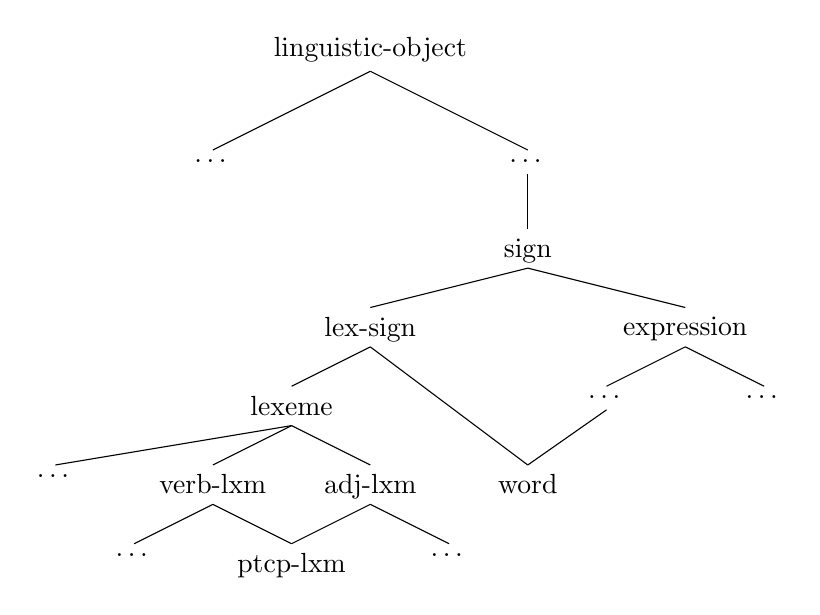
\begin{tikzpicture}

\draw (0,0) node[above]{linguistic-object};

\draw (0,0) -- (-2,-1);
\draw (-2,-1) node[below]{\ldots{}};
\draw (0,0) -- (2,-1);
\draw (2,-1) node[below]{\ldots{}};

\draw (2,-1.3) -- (2,-2);
\draw (2,-2) node[below]{sign};


\draw(2,-2.5) -- (4,-3);
\draw  (4,-3) node[below]{expression};
\draw(2,-2.5) -- (0,-3);
\draw  (0,-3) node[below]{lex-sign};

\draw(0,-3.5) -- (-1,-4);
\draw (-1,-4) node[below]{lexeme};
\draw(0,-3.5) -- (2,-5);
\draw (2,-5) node[below]{word};

\draw (4,-3.5) -- (3,-4);
\draw (3,-4) node[below]{\ldots{}};
\draw (4,-3.5) -- (5,-4);
\draw (5,-4) node[below]{\ldots{}};

\draw (3,-4.3) -- (2,-5);

\draw(-1,-4.5) -- (-4,-5);
\draw (-4,-5) node[below]{\ldots{}};
\draw(-1,-4.5) -- (-2,-5);
\draw (-2,-5) node[below]{verb-lxm};
\draw(-1,-4.5) -- (0,-5);
\draw (0,-5) node[below]{adj-lxm};

\draw(-2,-5.5) -- (-3,-6);
\draw  (-3,-6) node[below] {\ldots{}};
\draw(-2,-5.5) -- (-1,-6);
\draw  (-1,-6) node[below] {ptcp-lxm};

\draw(0,-5.5) -- (-1,-6);
\draw(0,-5.5) -- (1,-6);
\draw (1,-6) node[below] {\ldots{}};

%\draw(-5,-2.5) -- (-6,-3);
%\draw  (-6,-3) node[below]{gap};

\end{tikzpicture}
\caption{Revised partial \is{type hierarchy}type hierarchy} \label{fig:Spencer:types2}
\end{centering}
\end{figure}

This would be in keeping with %
%Malouf's
\citeauthor{Malouf00:book}'s %
%
 (\citeyear{Malouf00:book}) approach to deverbal nominalizations. However, there are a number of problems with this solution. One of these relates to the `directionality' or `headedness' of \is{transposition}transpositions: a \isi{transposition} is a representation of its base \is{lexeme}lexeme. In that respect a \is{participle}participial \isi{quasi-lexeme} bears the same relationship to a verb that, say, the past tense form bears. But this is not captured in a hierarchy such as that sketched in Figure \ref{fig:Spencer:types2}, where the relation between \textit{verb-lxm, adj-lxm}, the  two mothers of the \isi{participle} \textit{ptcp-lxm},  is equal. As a result, there will be no way of distinguishing between the adjectival \is{\textsc{representation} (feature)}representation of a verb and the verbal \is{\textsc{representation} (feature)}representation of an adjective (that is, a transpositional predicative adjective heading a finite clause and bearing inflections for verb features such as tense-mood-aspect-polarity or subject agreement).

 \newpage 
 \largerpage 
Perhaps, then we should adopt a different approach. Since \is{participle}participles are morphologically derived we can set up a construction type in \is{Sign-Based Construction Grammar}SBCG (or a lexical rule in standard \is{Head-driven Phrase Structure Grammar}HPSG) which would perform the same role as the GPF applied to the \is{\textsc{representation} (feature)}\textsc{repr} feature in \is{Generalized Paradigm Function Morphology}GPFM. Sag  defines two sorts of morphological construction relevant to us in this context, the \textit{infl-cxt}
and the \textit{deriv-cxt}.

\ea \label{ex:Spencer:infl-cxt}

\textit{infl-cxt}:		\begin{avm}
				\[mtr		&\textit{word}\\
				dtrs		&\textit{list}(\textit{lexeme})
				\]
				\end{avm}				
\hfill\citep[115]{Sag12}


\z\bigskip

\ea \label{ex:Spencer:deriv-cxt}

\textit{deriv-cxt}:
\begin{avm}
	\[mtr		&\textit{lexeme}\\
	dtrs		&\textit{list}(\textit{lex-sign})
	\]
\end{avm} 				
\hfill
\citep[119]{Sag12}%
%Sag
%

\z
The formulation in (\ref{ex:Spencer:deriv-cxt}) additionally permits derivation from word forms, but in general derivation is defined over \is{lexeme}lexemes and to simplify the discussion I will assume that this is always the case. If we take a \isi{participle} to be a subtype of \textit{\is{lexeme}lexeme}, then \isi{participle} formation will be a subtype of the derivational construction shown in~(\ref{ex:Spencer:deriv-cxt}).

One issue that has to be resolved when incorporating morphological models into lexicalist syntactic models arises from the fact that \is{inferential-realizational}I-R models of morphology are generally based on \is{default}default inheritance logic, while the syntactic models generally avoid the use of \is{default}defaults and overrides.  An important proposal for marrying the two systems is given by \citet{Bonami15} in the context of analysing \is{periphrasis}periphrastic constructions in Persian (see also \citealt{Bonami13}). The details depend on the specifics of their analysis, but the overall import of their proposal is a `meta-constraint' on signs of type \textit{word}, such that a word is licenced in the (\is{Head-driven Phrase Structure Grammar}HPSG) syntax only if a corresponding representation of it is also licensed in the (PFM) morphology %
%(Bonami and Samvelian 2014: 32)
\citep[32]{Bonami15}%
%
. In effect, they treat the PFM morphology as a `black box' whose outputs bear properties that can be recognized by the  syntax.

The interface for canonical inflection works well. However, the proposals do not touch directly on other types of morphology, notably derivation and \is{transposition}transpositions. Presumably, the interface principle could be extended so as to apply between a morphological engine and the \is{Head-driven Phrase Structure Grammar}{HPSG} lexicon. A major problem here is the lack of consensus over how to handle derivational morphology in \is{inferential-realizational}I-R models.  In PFM there has been very little discussion of derivation and no discussion of \is{transposition}transpositions.%
\footnote{This includes %
%Stump (2016a, b)
\citet{Stump16,Stump16:MorphMetatheory}%
%Stump
%
\nocite{Stump16,Stump16:MorphMetatheory}, which are concerned exclusively with \textsc{form/content} mismatches.} %
Concrete proposals for derivation and \is{transposition}transpositions can be found in the Network Morphology model of %Brown and Hippisley (\citeyear{Brown:Hippisley12:book})%
 \citet{Brown:Hippisley12:book}  but it is not clear how that model would interface with syntax. Moreover, it is not clear how the Network Morphology model distinguishes between \is{transposition}transpositions and canonical derivation, and between these and the (non-canonical) phenomenon of \is{transpositional lexeme}transpositional lexemes.


\begin{sloppypar}
A detailed set of proposals for defining lexical relatedness is given in %
%Spencer (2013)
\citet{Spencer13}%
%Spencer
%
, where I show that there are many other types of relatedness between words in addition to canonical inflection, canonical derivation and true (canonical) \is{transposition}transposition. Any model of the lexicon has to be able to account for all these types. They include meaning-changing inflection,  meaning-changing \is{transposition}transposition, derivation which involves no change at all in \textsc{form} properties (morphologically inert derivation) and others. The conceptual problem here is that any of these types of relatedness might be part of the paradigmatic grammatical system in a given language, in which case the morphological means by which they are all expressed cannot be distinguished. Therefore, the same kind of machinery has to be deployed for paradigmatic derivation as for inflection. Given our current assumptions this means some form of \is{paradigm function}paradigm function, defined in terms of \is{default}defaults and overrides, and the challenge is therefore to ensure that the \is{lexical representation}lexical representations so defined are compatible with the kinds of representations deployed in the syntax.
\end{sloppypar}





%An agenda for lexical representation

\section{An agenda for \is{lexical representation}lexical representation} \label{sec:Spencer:agenda}

The foregoing discussion raises more question than it answers, but the questions are important for lexicalist, constraints-based models generally, and for theories of \is{lexical representation}lexical representation and morphology generally. Here, by way of a conclusion I summarize the main issues that have emerged.

\begin{itemize}

\item	Are \is{lexeme}lexemes partially specified linguistic objects?

\item	What is the relationship between \is{transposition}transpositional \is{quasi-lexeme}quasi-lexemes and canonical \is{lexeme}lexemes?

\item		How do we ensure that \is{inferential-realizational}I-R morphological models can interface with constraints-based syntactic models, including all aspects of paradigmatically organized morphology?

\item	To what extent can the morphological functions/constructions proposed in %
%Sag (2012) 
\citet{Sag12} %
%Sag
%
be retained in their current form? To what extent can such constructional types, or their more traditional incarnations in standard \is{Head-driven Phrase Structure Grammar}HPSG, be made compatible with \is{inferential-realizational}I-R models?

\end{itemize}

Finally, the most difficult question of all is the oldest and the one with the widest significance: what kind of a thing is a dictionary entry? Is it a real, mentally represented linguistic construction or is it merely the convenient fiction of the lexicographer? We cannot address this question without providing very explicit answers to the representational and ontological questions raised in this paper, and so I present my discussion of those questions as a modest contribution towards answering the much bigger question.








%%%%%%%	 ABBREVIATIONS	%%%%%%%
\section*{Abbreviations}

\begin{tabular}{ll}
\textsc{arg-st}		&Argument Structure (attribute)\\
FS 			&feature structure\\
GPFM     		&Generalized Paradigm Function Morphology\\
HPSG	     		&Head-driven Phrase Structure Grammar\\
I-R     			&inferential-realizational (model)\\
\textsc{li}			&Lexical/Lexemic Index\\
\textsc{lid}			&Lexical Identifier\\
PFM     		&Paradigm Function Morphology\\
SBCG     		&Sign-Based Construction Grammar\\
SF     			& semantic function (role)\\
wfr			&Word Formation Rule
\end{tabular}

 {\sloppy
 \printbibliography[heading=subbibliography,notkeyword=this]
 }
\end{document}
